\chapter{TRABALHOS RELACIONADOS}
\label{chp:relatedWorks}

O presente capítulo apresenta o estado da arte em relação à ferramentas de busca de código-fonte. Os trabalhos apresentados nesses capítulo estão ordenados em ordem cronológica de publicação. Por fim, é apresentada também uma conclusão sobre os trabalhos citados neste capítulo.

\textcite{Sadowski2015HowDS} realizaram um estudo empírico entre desenvolvedores da empresa Google para analisar padrões de busca de código. O estudo foi realizado utilizando duas ferramentas: um questionário com cinco perguntas, que era apresentado ao usuário sempre que este acessava o repositório interno da empresa; e a coleta de registros (logs) gerados por uma ferramenta de busca de código, utilizada pelos usuários do estudo. Os resultados mostraram que programadores realizam, em média, cinco sessões de busca de código, com doze consultas por sessão, por dia de trabalho. Além disso, tais consultas são, geralmente, relacionadas aos seguintes pontos: uso de API; o que o código faz; porque o código está falhando; onde o código está localizado. Como trabalhos futuros, os autores apontam algumas áreas que não foram contempladas pelo estudo em questão, como a qualidade dos resultados da busca e de que forma os resultados da busca são utilizados pelo usuário. 

\textcite{lv2015codehow} notaram que as ferramentas de busca de código existentes tinham dificuldades com consultas em linguagem natural. Por isso, os autores propuseram a \textit{CodeHow}: uma ferramenta de busca de código que utiliza o modelo booleano extendido. Este modelo avalia a similaridade do texto da consulta com a documentação do código, a fim de ranquear os resultados da consulta em questão. Os autores conduziram o estudo com vinte desenvolvedores e estagiários da empresa Microsoft. Ao final, a \emph{CodeHow} obteve $0,794$ utilizando a métrica \textit{Precision@1}, e $0,867$ com a métrica \gls{mrr}. Tais resultados superaram as ferramentas existentes durante o período do estudo, como Ohloh e Apache Lucene. Contudo, os autores levantaram que, como a \textit{CodeHow} não consegue compreender os significados semânticos da consulta e do código, algumas consultas retornaram resultados incorretos. Um exemplo é a consulta "converter uma cor de RGB para HSV", para a qual a \textit{CodeHow} retornava resultados relevantes à consulta "converter uma cor de HSV para RGB". 

\textcite{Gu2018DeepCS} propuseram uma rede neural profunda, chamada \textit{CODEnn}, capaz de relacionar trechos de código com consultas em linguagem natural. Além disso, os autores criaram uma ferramenta de busca de código (\gls{deepcs}), baseada na \textit{CODEnn}, como prova de conceito do estudo em questão. Para relacionar linguagem natural com código, a \textit{CODEnn} aprende as representações vetoriais do par código/descrição, de forma que um trecho de código é relacionado à uma consulta em linguagem natural utilizando o vetor gerado pela consulta. Utilizando este método, os autores obtiveram resultados de busca de código melhores do que ferramentas como Apache \textit{Lucene} e \textit{CodeHow}. Por fim, como trabalhos futuros, os autores pretendem investigar mais aspectos de códigos-fontes, como estruturas de controle, a fim de melhorar a representação de semânticas de alto nível do código-fonte.

\textcite{Chu2019AGA} propôs um sistema para busca de código que combina aprendizagem de máquina baseada em grafos com modelos \emph{transformer}, além de modelos tradicionais de busca como \textit{ElasticSearch} (ferramenta de busca baseada no Apache \textit{Lucene}). O sistema em questão aplicou \emph{embeddings} hiperbólicos e clusterização de grafos aos dados da base \emph{CodeSearchNet} \cite{Husain2019CodeSearchNetCE}, a fim de incorporar a estrutura de grafos presente nos repositórios de código aos modelo de busca testados. Com isso, foram testados os seguintes modelos de busca: \gls{nbow}; \textit{ElasticSearch}; \textit{ElasticSearch} com clusterização de grafos. Utilizando a métrica \gls{ndcg}, comumente utilizada para avaliar mecanismos de busca, obteve-se $0,190$ com o \gls{nbow}, $0,196$ com \textit{ElasticSearch} e $0,208$ com o \textit{ElasticSearch} com clusterização de grafos. Por fim, dentre as melhorias sugeridas pelos autores está a utilização de outros modelos neurais no lugar do \textit{ElasticSearch}, combinados com o modelo de grafos proposto.

\textcite{Cambronero2019WhenDL} analisaram o uso de modelos de aprendizado supervisionado e não supervisionado dentro do contexto de busca de código. Para tanto, os autores criaram uma plataforma comum de testes, e utilizaram \textit{benchmarks} como \gls{mrr}, além de criarem um modelo supervisionado, chamado \gls{unif}, o qual consiste em uma variação de um modelo \gls{ncs} (não supervisionado). Nos testes, os autores obtiveram resultados melhores com modelos supervisionados do que com modelos não supervisionados. Com isso, os autores sugerem o uso modelos de aprendizagem mais simples (como o \gls{unif}) para sistemas de busca de código. Além disso, o estudo mostra que uma base de dados de treinamento que se assemelhe com consultas comuns dos usuário, provê melhorias significativas para todos os modelos supervisionados.

\textcite{Wan2019MultimodalAN} propuseram o modelo \gls{mman} para busca semântica de código. O \gls{mman} utiliza diversos outros modelos, como \gls{lstm}, \textit{Tree-LSTM} e \gls{ggnn}, para representar características do código-fonte. O estudo em questão comparou o \gls{mman} com outros métodos de busca de código (como \textit{CodeHow} e \gls{deepcs}) utilizando as métricas \textit{SuccessRate@k} e \gls{mrr}, além de dados disponíveis no \textit{Github} para criação da base de dados. Com isso, o \gls{mman} obteve os melhores resultados no estudo. Como trabalhos futuros, os autores planejam aplicar o \gls{mman} em outras tarefas de engenharia de software como sumarização de código e detecção de plágio em código-fonte.

\textcite{Yao2019CoaCorCA} propuseram um modelo de aprendizagem por reforço, chamado \gls{coacor}, o qual gera descrições (em linguagem natural) de código-fonte a fim de melhorar modelos de busca de código. Os testes do estudo foram realizados com a base de dados \textit{StaQC} \cite{Yao2018StaQCAS} e utilizando os modelos de busca de código \gls{deepcs} e \textit{CODEnn}, além do \gls{mrr} e \gls{bleu} como métricas para busca de código e geração de descrição, respectivamente. Os resultados mostraram que o \gls{coacor} foi capaz de gerar descrições úteis para trechos de código, e que tais descrições foram capazes de melhorar a performance dos modelos de busca testados.

\textcite{Akbar2019SCORSC} estudaram a combinação de \glspl{cam} com a semântica dos vetores de palavras obtidos pelo algoritmo \textit{word2vec}. Com isso, os autores compararam as sequências de palavras de uma consulta em linguagem natural, e de um código-fonte. Utilizando as métricas \textit{MAP}, \textit{Precision@k} e \textit{Recall@k}, além das bases de dados \textit{BUGLinks} e \textit{iBUGS}, o estudo em questão obteve melhoras entre $6\%$ e $30\%$ de acurácia na busca de código.

\textcite{Heyman2020NeuralCS} estudaram o impacto que códigos anotados tem em modelos de busca de código. Segundo os autores, um código anotado é um trecho de código com descrições de sua intenção em linguagem natural. Durante o estudo, foram utilizados os modelos de busca de código \gls{ncs} e \gls{unif}, além das bases de dados \textit{CoNaLa}, \textit{StaQC} \cite{Yao2018StaQCAS} e SO-DS, as quais contém códigos em \emph{Python}. Como \emph{benchmark}, foram utilizadas as métricas \textit{recall@3}, \textit{recall@10} e \gls{mrr}. Ao se utilizar código anotado, obteve-se uma melhora de $20.6\%$ no \gls{mrr}, $23,9\%$ no \textit{recall@3} e $26,4\%$ no recall@10, em comparação aos métodos de busca que não utilizam código anotado. Por fim, os autores acreditam que tais melhorias poderão ser notadas mesmo como outras linguagem de programação (como Java, por exemplo), caso seja aplicado o uso de código anotado nos modelos de busca.

\textcite{Yan2020AreTC} observaram dificuldades em se comparar métodos de busca de código, como a falta de uma bases de dados em comum para comparação de dois métodos de busca. Diante disso, os autores realizaram um estudo empírico para comparação de dois tipos de métodos de busca de código a partir de consultas em linguagem natural. Os dois tipos de método em questão são: métodos baseados em \gls{ir}, e baseados em \gls{dl}. Para tanto, os autores criaram uma base de dados com códigos Java, chamada \textit{CosBench}, e utilizaram essa base para comparar quatro métodos de busca \gls{ir} e dois métodos \gls{dl}. Por fim, os resultados mostraram que os métodos baseados em aprendizagem profunda são mais adequados para consultas relacionadas à reutilização de código, enquanto métodos baseados em recuperação de informação são mais adequados para consultas relacionadas à resolução de \emph{bugs} e usos de determinadas \glspl{api}. Como trabalhos futuros, os autores levantam que a intenção da consulta feita pelo programador possa ser inferida automaticamente, de forma a ajudá-lo a encontrar o melhor método de busca para sua consulta.

\textcite{Feng2020CodeBERTAP} propuseram o \textit{CodeBERT}, um modelo bimodal para linguagem de programação e linguagem natural. O \textit{CodeBERT} utiliza uma arquitetura baseada no modelo \gls{bert}. Porém, o \textit{CodeBERT} é capaz de aceitar tanto dados bimodais (par código/linguagem natural) quanto dados unimodais (apenas código). Dados bimodais geralmente são usados para tarefas de busca de código, enquanto dados unimodais para geração de código. Com o \textit{CodeBERT}, os autores conseguiram resultados iguais ou, em alguns casos, melhores do que o estado da arte. As comparações foram feitas utilizando as métricas \gls{mrr} para busca de código e \gls{bleu} para geração de código. Por fim, como trabalhos futuros, os autores apontam a incorporação de \gls{ast} nas fases de pré-treino.

\textcite{Li2020LearningCI} propuseram o \gls{cqil}, um modelo de busca de código que utiliza redes neurais convolucionais para encontrar relações léxicas e semânticas entre a consulta e o trecho de código. A fim de comparação, o estudo utilizou os modelos de busca \gls{deepcs}, \gls{unif}, Apache Lucene e \textit{CodeHow}, bem como as métricas \textit{map@k}, \textit{SuccessRate@k} e \gls{mrr}, além das base de dados \textit{CODEnn} e \textit{CosBench}. Os experimentos realizados mostraram melhora de performance em todas as métricas utilizadas. Além disso, os autores apontam que o \gls{cqil} também possui boa performance com bases de dados pequenas.

\textcite{Ye2020LeveragingCG} utilizaram geração de código para melhor correlacionar linguagem de programação e linguagem natural. Para tanto, o modelo proposto, chamado \gls{co3}, utiliza \textit{dual
learning} e \textit{multi-task learning}. Para os experimentos, os autores utilizaram o banco de dados \textit{StaQC} \cite{Yao2018StaQCAS}, o qual contém trechos de código das linguagens de programação \gls{sql} e \textit{Python}. Utilizando as métricas \gls{mrr} e \gls{ndcg}, os autores obtiveram $0,585$ e $0.682$ (respectivamente) para \gls{sql}, e $0,679$ e  $0,756$ para \textit{Python}. Como trabalhos futuros, os autores planejam explorar as interações entre as perdas de ranking para busca de código.

\textcite{Ling2020AdaptiveDC} propuseram um método de busca de código chamado \gls{adacs}. Este método divide o processo de aprendizagem em duas etapas: aprendizagem de \textit{embeddings} de domínio específico, e aprendizagem de combinações de padrões sintáticos. Isso possibilita ao \gls{adacs} se adaptar à novas palavras, específicas de determinado domínio, mesmo que estas não tenham sido aprendidas durante o treinamento. Para os experimentos, o estudo utilizou códigos escritos em \textit{Java} e disponíveis no \textit{Github} e métodos de busca de código como \textit{CodeHow} e \gls{deepcs}. Utilizando as métricas \gls{mrr} e \textit{hit@k}, o \gls{adacs} obteve resultados melhores em todas as comparações feitas no estudo. Por fim, dentre os possíveis trabalhos futuros, os autores planejam melhorar a eficiência de tempo do \gls{adacs} utilizando \textit{encoders} transformers.

\textcite{Wang2020TranS3AT} propuseram o $TranS^3$, o qual consiste em um modelo, baseado em redes \textit{transformer}, para integração de sumarização de código e busca de código. O $TranS^3$ é capaz de gerar comentários para determinado trecho de código. Com isso, utilizando os comentários gerados, o $TranS^3$ consegue melhorar o treinamento para busca de código, relacionando assim trechos de código com linguagem natural. A fim de avaliar a performance de busca de código, o estudo utilizou as métricas \gls{mrr}, \textit{SuccessRate@k} e \gls{ndcg}, bem como diversos modelos de busca de código como \gls{deepcs}, \textit{Hybrid-DeepCom} e \gls{coacor}. Dos resultados, observa-se que o $TranS^3$ obteve performance semelhante ou melhor do que todos os modelos comparados, tanto na tarefa de busca de código quanto de sumarização de código.

\textcite{Guo2021GraphCodeBERTPC} desenvolveram o \gls{graphcodebert}: um modelo \textit{transformer} pré-treinado para linguagens de programação, que considera a estrutura inerente do código-fonte. Para tanto, ao invés de usar estruturas sintáticas de código como a \gls{ast}, o \gls{graphcodebert} utiliza o \textit{data flow}. O \textit{data flow} consiste em uma representação de código-fonte, a qual é menos complexa do que \gls{ast}, e contém informações sobre as relações entre as variáveis utilizadas no código. O estudo testou o \gls{graphcodebert} em tarefas relacionadas à linguagem de programação, incluindo busca de código a partir de linguagem natural. Para esta tarefa em específico, os autores utilizaram a métrica \gls{mrr}, o banco de dados \textit{CodeSearchNet} \cite{Husain2019CodeSearchNetCE} e sete modelos de busca de código, incluindo \gls{nbow}, \gls{birnn}, \textit{RoBERTa}, \textit{CodeBERTa} e \textit{CodeBERT}. Em todas as comparações, os autores notaram que o \gls{graphcodebert} obteve resultados melhores na tarefa de busca de código a partir de linguagem natural.

\textcite{Xu2021TwoStageAM} propuseram um modelo de busca de código chamado \gls{tabcs}, o qual consiste em um modelo de atenção de duas etapas: a primeira extrai dados semânticos tanto do código quanto da consulta, enquanto a segunda etapa detecta as relações semânticas entre código e consulta, a fim de aprender representações melhores dessas duas entidades. Em comparação com os modelos \gls{carlcscnn}, \gls{deepcs} e \gls{unif}, o \gls{tabcs} obteve uma melhora de $18\%$, $70\%$ e $12\%$ no \gls{mrr} respectivamente. Como trabalhos futuros, os autores planejam incorporar outras características do código-fonte, como estruturas de controle de fluxo, a fim de melhorar a representação do código-fonte.

\textcite{Bui2021SelfSupervisedCL} propuseram um modelo de aprendizagem auto-supervisionado contrastante para modelagem de código-fonte chamado \textit{Corder}. Este modelo pode ser usado tanto para produzir a rotulação de dados, as quais são aplicadas em sumarização de código, quanto para produzir representações  vetoriais de código-fonte, utilizadas em tarefas de busca de código. Para os experimentos relacionados à busca de código a partir de texto (\textit{text-to-code}), utilizou-se a base de dados disponível em \cite{Gu2018DeepCS}. Para comparação, foram utilizadas as métricas \textit{Precision@k} e \gls{mrr}, além dos modelos transformer, \gls{nbow}, \gls{tbcnn} e \gls{bilstm}. Em todos os experimentos realizados, os autores observaram melhoras no resultados dos modelos que utilizaram o \textit{Corder}, em relação aos que não utilizaram.

\textcite{Gu2021CRaDLeDC} propuseram um modelo de representação de código-fonte chamado \gls{cradle}. Este modelo combina as informações semânticas e de dependência contidas na instrução do código, a fim de gerar uma representação vetorial unificada para cada par código/descrição. O estudo utilizou as bases de dados \textit{CodeSearchNet} \cite{Husain2019CodeSearchNetCE} e \textit{Code2Sec}. Além disso, utilizou-se as métricas \textit{R@k} e \gls{mrr}, e os modelos de busca de código \textit{CODEnn}, \gls{unif} e \gls{nbow} para comparação de performance. Dos resultados, obteve-se melhoras em todas as métricas com a utilização do \gls{cradle}. Como trabalhos futuros, os autores pretendem incorporar, ao treinamento da rede, conhecimentos externos ao código, como documentação de \glspl{api}, a fim de melhorar a representação semântica do código-fonte.

\textcite{Liu2021GraphSearchNetEG} desenvolveram o modelo de busca de código \textit{GraphSearchNet}. Este modelo utiliza uma \gls{gnn} bidirecional para representar as informações estruturais tanto das consultas quanto do código-fonte. Além disso, o modelo proposto utiliza um módulo de atenção múltipla para suplementar as dependências globais dos grafos gerados. O \textit{GraphSearchNet} foi comparado com diversos modelos de busca (como \gls{deepcs}, \gls{unif} e \gls{nbow}), utilizando as métricas \textit{SuccessRate@k}, \gls{ndcg} e \gls{mrr}, além da base de dados \textit{CodeSearchNet} \cite{Husain2019CodeSearchNetCE}, utilizando os dados linguagens \textit{Python} e \textit{Java} para o estudo em questão. Por fim, a \textit{GraphSearchNet} obteve resultados melhores em todas as métricas utilizadas. Além disso, a \textit{GraphSearchNet} obteve uma performance melhor na linguagem \textit{Python}. Isso se deu, segundo os autores, porque \textit{Python} possui recursos gramaticais mais simples e uma distância semântica (\textit{semantic gap}) menor, quando comparada ao \textit{Java}.

\textcite{Zeng2021deGraphCSEV} notaram que as ferramentas de busca de código que utilizam aprendizagem de máquina são limitadas pelas técnicas de representação e modelagem do código-fonte. Portanto, os autores propuseram a \gls{degraphcs}, capaz de converter código-fonte em grafos de fluxo baseado em variáveis, a fim de modelar a semântica do código de forma mais precisa do que \gls{ast}. Como trabalhos futuros, os autores apontam otimizações para remoção de informações redundantes nos grafos gerados.

\textcite{Du2021IsAS} perceberam que um trecho de código contém diferentes características, como lógica de negócio e comunicação com \textit{hardware}, de forma que seria difícil um único modelo representar todas essas dimensões. Com isso, os autores propuseram a \textit{MuCoS}, uma arquitetura de aprendizagem multimodal para busca semântica de código. Nessa arquitetura, ao invés de um módulo de aprendizagem para descrever todas as características do código, há múltiplos módulos de aprendizagem, um para cada característica. Depois, os autores utilizam técnicas de aprendizagem por agrupamento (\textit{ensemble learning}) para combinar todos os módulos. Para os testes, os autores utilizam a base de dados \textit{CodeSearchNet} \cite{Husain2019CodeSearchNetCE} e as métricas \textit{SuccessRate@k} (com $k=1$, $k=5$ e $k=10$) e \gls{mrr}. Utilizando tais métricas, o \textit{MuCoS} obteve $0,750$, $0,843$, $0,860$ e $0,793$, respectivamente. O segundo melhor modelo testado no estudo, \textit{CodeBERT}, obteve $0,642$, $0,792$, $0,825$ e $0,708$, respectivamente. Por fim, os autores planejam implementar um módulo de seleção para ajudar a escolher modelos de aprendizagem específicos para determinada busca.

\textcite{Ling2021DeepGM} propuseram um modelo para busca semântica de código-fonte chamado \gls{dgms}. Esse modelo representa tanto textos em linguagem natural quanto trechos de códigos com uma estrutura unificada de grafos. O estudo avaliou o \gls{dgms} utilizando as bases de dados \textit{FB-Java} e \textit{CSN-Python}. Além disso, os autores compararam o \gls{dgms} com os modelos \gls{nbow}, \gls{deepcs}, \gls{unif} e \textit{CAT} \cite{Haldar2020AMA}, utilizando as métricas \gls{mrr} e \textit{SuccessRate@k}. Por fim, o estudo mostrou que o \gls{dgms} obteve resultados consideravelmente melhores do que os outros modelos, nas duas métricas utilizadas no estudo em questão. Além disso, os autores planejam explorar outras formar de construir grafos de texto e código para outras linguagem de programação, como C\#.

\textcite{Salza2021OnTE} estudaram a aplicação de modelos \textit{transformers} em busca de código. Para tanto, os autores utilizaram dados do \textit{Stack Overflow} e do \textit{GitHub} para gerar bancos de dados de diversas linguagens de programação, como \textit{JavaScript}, \textit{Java} e \textit{Python}. Além disso, utilizou-se um modelo \textit{transformer} baseado no \gls{bert}, e as métricas \gls{mrr}, \textit{Aroma} e \textit{Top-k}. Com isso, o estudo concluiu que a transferência de conhecimento, possibilitada pelos modelos \textit{transformers}, é um método efetivo para melhorar a performance de busca de código em redes neurais. Entretanto, pelo fato dos modelos \textit{transformers} demandarem uma quantidade significativa de recursos computacionais, o estudo sugere a utilização de outros modelos de busca de código, como \textit{Apache Lucene}, para bases de dados pequenas. Por fim, no estudo em questão os autores utilizaram o modelo \gls{bert}, que analisou o código como uma sequência de \textit{tokens}. Entretanto, os autores sugerem que os resultados obtidos pelo BERT seriam melhores caso este fosse capaz analisar a estrutura do código, como a \gls{ast} por exemplo.

\textcite{Chai2022CrossDomainDC} propuseram um modelo chamado \gls{cdcs}. Diferente do \textit{CodeBERT} que precisa ser treinado na linguagem de código alvo, o \gls{cdcs} é pré-treinado com uma grande base de dados de determinada linguagem, como \textit{Java} ou \textit{Python}. Então, utilizando o algoritmo de meta-aprendizagem \textit{MAML}, o \gls{cdcs} se adapta a linguagem alvo que, no caso do estudo em questão, foi \gls{sql} e \textit{Solidity}. Os experimentos do estudo foram avaliados utilizando as métricas \gls{mrr} e top-k, e mostraram que o \gls{cdcs} atingiu melhoras significativas no domínio de busca de código, quando comparado com outros modelos como \textit{CodeBERT} e \textit{GPT2}. Por fim, os autores pretendem investigar a aplicação do \gls{cdcs} com outras linguagem de programação, além de aplicar o \gls{cdcs} em outras tarefas de engenharia de software.

\textcite{Sun2022CodeSB} propuseram um modelo de busca de código chamado \textit{TranCS}. Primeiro, o \textit{TranCS} utiliza uma técnica de tradução de código para linguagem natural baseada em contexto. Depois, o \textit{TranCS} utiliza uma função de mapeamento a fim gerar \textit{embeddings} tanto para as traduções quanto para as buscas de código. Tanto a técnica de tradução quanto a função de mapeamento foram desenvolvidas pelos autores.
Com isso, os autores compararam o \textit{TranCS} com os modelos \gls{deepcs} e \gls{mman}, utilizando a base de dados de \cite{Husain2019CodeSearchNetCE} e a métrica \gls{mrr}. Os resultados mostraram que o \textit{TranCS} obteve melhoras de $49,31\%$ a $66,50\%$ em relação aos outros modelos utilizados no estudo. Como trabalhos futuros, os autores citaram a construção de representações para longos trechos de código (acima de 20 linhas, segundo os autores).

\textcite{Sun2022OnTI} propuseram um sistema para redução de ruído em bases de dados de busca de código. Tal sistema consiste em dois filtros subsequentes: um filtro sintático e um semântico. Nos experimentos, os autores utilizam o modelo de busca \gls{deepcs} para comparação, bem como as métricas \gls{mrr} e \textit{Answered@k} (com k = 1), além de dados disponíveis em \cite{Husain2019CodeSearchNetCE} e no GitHub. Com isso, observou-se uma média de $19,2\%$ e $21,3\%$ nas métricas \gls{mrr} e \textit{Answered@k}, respectivamente.

\textcite{Shi2022EnhancingSC} desenvolveram um modelo para busca de código que utiliza aprendizagem multimodal contrastiva e \textit{soft data augmentation} chamado \textit{CoCoSoDa}. A \textit{soft data augmentation} é obtida mascarando e substituindo alguns \textit{tokens} na sequências de código para gerar trechos de código que são similares, mas que não necessariamente preservam a relação semântica entre o par código/consulta. Os experimentos do estudo utilizaram as métricas \gls{mrr} e \textit{SuccessRate@k}, e a base de dados \textit{CodeSearchNet} \cite{Husain2019CodeSearchNetCE}. Para comparação de performance, foram utilizados os modelos \gls{nbow}, redes neurais convolucionais, redes neurais recorrentes bidirecionais e \textit{SelfAtnn}. Os experimentos também testaram a aplicação do CoCoSoDa para melhorar a performance de modelos de atenção. Os modelos de atenção testados foram \textit{RoBERTa}, \textit{CodeBERTa},
\textit{CodeBERT} e \gls{graphcodebert}. Os resultados mostraram que o \textit{CoCoSoDa} obteve uma performance melhor do que os modelos testados. Além disso, os modelos de atenção que utilizam o CoCoSoDa também apresentaram melhoras de performance. Como trabalhos futuros, os autores pretendem convidar desenvolvedores para avaliar a relação semântica entre trechos de código e consultas em linguagem natural.

\textcite{Wang2022EnrichingQS} propuseram \gls{quecos}, um modelo de aprendizagem por reforço para busca de código. O estudo utilizou as bases de dados \textit{CodeSearchNet} \cite{Husain2019CodeSearchNetCE} e \textit{SOTorrent}. Além disso, para comparação utilizou-se as métricas \textit{SuccessRate@k} e \gls{mrr}, e os modelos de busca de código \gls{deepcs}, \gls{unif}, \textit{OCoR} e \textit{CodeBERT}. Dos resultados, nota-se que o \gls{quecos} obteve resultados melhores do que os modelos comparados, em todas as métricas consideradas no estudo. Como trabalhos futuros, os autores planejam utilizar bases de dados maiores para o treinamento, além de incorporarem grafos de conhecimento externos para melhorar a semântica das buscas.

\textcite{Gu2022AcceleratingCS} propuseram um modelo de busca de código, baseado em \textit{deep hashing} e classificação de código, chamado \gls{coshc}. O estudo utilizou dois bancos de dados de código em \textit{Python} e \textit{Java}, ambos providos por \cite{Feng2020CodeBERTAP}. Para comparação, foram utilizados os modelos \gls{unif}, \gls{rnn}, \textit{CodeBERT}, \textit{CodeBERTa} e \textit{GraphCodeBERT}, além da métrica \textit{SuccessRate@k}. Os resultados mostraram que o \gls{coshc} foi melhor em comparação ao modelos \gls{unif} e \gls{rnn}, mas obteve resultados iguais ou piores na maioria dos testes com \textit{CodeBERT}, \textit{CodeBERTa} e \textit{GraphCodeBERT}.

\textcite{Cheng2022CSRSCS} propuseram um modelo de busca de código chamado \gls{csrs}, o qual consiste de três partes principais: um módulo de \textit{embedding} com núcleos de convolução para extrair \textit{embeddings} n-gramas de consultas e códigos; um módulo para medir as correspondências léxicas das consultas; e um módulo baseado em atenção para capturar a correlação semântica entre consulta e código. Utilizando a métrica \gls{mrr}, e a base de dados utilizada em \cite{Gu2018DeepCS}, o \gls{csrs} obteve melhora de $33,77\%$ e $18.53\%$ em relação aos modelos \gls{deepcs} e \gls{carlcscnn}. Como trabalhos futuros, os autores consideram estudar formas de melhorar a combinação dos módulos do \gls{csrs}, além de incorporar conhecimento externo (como \gls{ast} ou documentação de \gls{api}) ao treinamento do \gls{csrs}.

\section{Conclusões do Capítulo}
O gráfico da Figura \ref{fig:related-datasets} mostra as bases de dados utilizadas nos estudos analisados. Nota-se que a grande maioria das bases utiliza dados disponíveis ou no \textit{Github} (\textit{CodeSearchNet} e \textit{CosBench}) ou no \textit{Stack Overflow} (\textit{StaQC}). O fácil acesso, grande volume de dados e a forma como os dados estão estruturados podem ser explicações para o uso dessas duas fontes de dados. Inclusive, essa estruturação é especialmente relevante no caso do \textit{Stack Overflow}. Além das respostas dos usuários normalmente conterem tanto um trecho de código-fonte quanto sua explicação em linguagem natural, há também um sistema de votação, fazendo com que as respostas mais relevantes tenham mais votos dos usuários.
\begin{figure}[H]
    \centering
    \caption{Bases de dados utilizadas}
    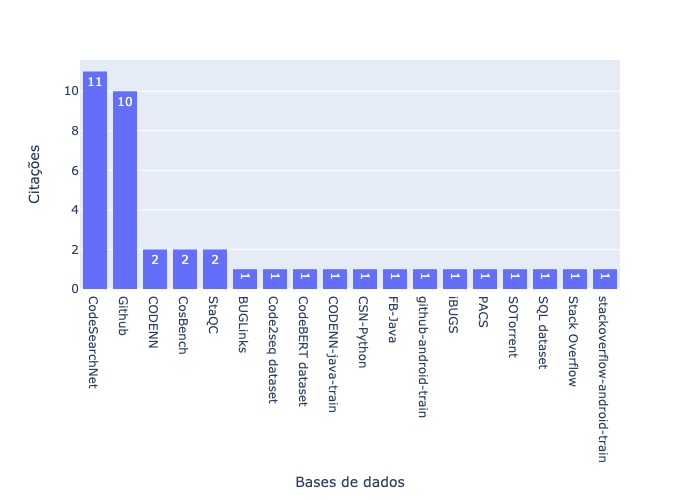
\includegraphics[width=1.0\columnwidth, height=0.6\columnwidth]{./imagens/trabalhos-relacionados/databases.png}
    \smallcaption{Fonte: Autor}
    \label{fig:related-datasets}
\end{figure}

O gráfico da Figura \ref{fig:related-metrics} mostra as métricas utilizadas nos estudos em questão. Nota-se que \gls{mrr} e \textit{SuccessRate@k} foram as métricas mais utilizadas para o problema de busca de código.
\begin{figure}[H]
    \centering
        \caption{Métricas utilizadas}
        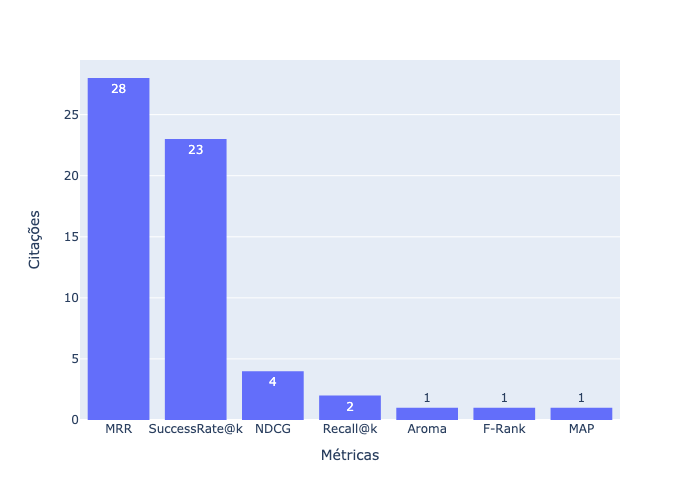
\includegraphics[scale=0.5]{./imagens/trabalhos-relacionados/ir_metrics.png}
        \smallcaption{Fonte: Autor}
        \label{fig:related-metrics}
\end{figure}

A Figura \ref{fig:related-baselines} mostra os modelos de busca de código utilizados como base de comparação nos estudos em questão. Nota-se que a maioria dos modelos utilizam redes neurais profundas, com exceção do \gls{unif}, \textit{Apache Lucene} e \textit{ElasticSearch}. Além disso, nota-se o uso extensivo de modelos \textit{transformers} baseados em \gls{bert}, como \textit{CodeBERT}, \textit{RoBERTa} e \textit{GraphCodeBERT}. Uma possível explicação para o uso de modelos \textit{transformers} é a eficiência de tais modelos quando comparados com outras técnicas como busca textual ou redes neurais profundas.
\begin{figure}[H]
    \centering
        \caption{Modelos de comparação utilizados}
        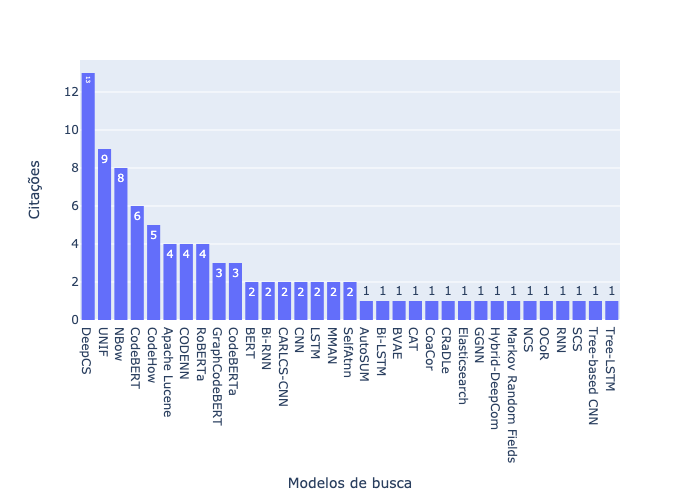
\includegraphics[scale=0.5]{./imagens/trabalhos-relacionados/baselines.png}
        \smallcaption{Fonte: Autor}
        \label{fig:related-baselines}
\end{figure}

Portanto, a fim de determinar qual o melhor modelo apresentado, concluímos que não é possível realizar tal comparação utilizando os resultados apresentados em seus respectivos estudos. Isso porque, apesar dos experimentos utilizarem as mesmas métricas de busca, os resultados dependem de fatores específicos dos estudos em questão, como a base de dados utilizada.
